\documentclass[10pt,letterpaper]{article}
\usepackage[utf8]{inputenc}
\usepackage{amsmath}
\usepackage{amsfonts}
\usepackage{amssymb}
\usepackage{graphicx}
\usepackage[left=2cm,right=2cm,top=2cm,bottom=2cm]{geometry}
\author{Darrel J. Conway\\Thinking Systems, Inc.}
\title{Assignment to Cloned Objects in Command Mode}
\begin{document}
\maketitle
\begin{abstract}
This document describes the structures and interfaces used in the General Mission Analysis Tool (GMAT) to support parameter setting on configured objects that are cloned as members of other objects.  The document is written and formatted in a style that facilitates inclusion in the GMAT Architectural Specification.
\end{abstract}

\section{Introduction}

When GMAT loads and runs a script, it performs this action is several distinct stages.  The script loading process takes a text description of GMAT's objects needed for the mission and converts that serialized version of the mission into the objects needed to model the mission.  The script file is usually configured with the descriptions of mission resources at the top of the file, followed by a description of the mission time line in the form of a sequence of commands comprising the Mission Control Sequence.  The script parsing runs in two separate modes, called ``Object Mode'' and ``Command Mode.''  The distinction is made between these modes so that parameter settings that should only be applied at a specific point inside of the Mission Control Sequence can be applied at that scripted location in the time line.  As an example, consider the following partial script:
\begin{quote}
\begin{verbatim}
Create Spacecraft sat;
Create Propagator prop;

BeginMissionControlSequence;

Propagate prop(sat) {sat.Periapsis};
sat.VX = 2.0;
Propagate prop(sat) {sat.Apoapsis};
sat.VX = -1.5;
Propagate prop(sat) {sat.ElapsedDays = 2};
\end{verbatim}
\end{quote} 

\noindent For this scripting, the user clearly wants the value of sat.VX to change at specific times on the time line, and not to be applied as values on the Spacecraft object when the script is translated into GMAT objects.

When a script is deserialized into GMAT objects, those objects are placed in separate collections in memory.  Named GMAT Resources are stored in a table managed by GMAT's configuration manager.  Commands in the Mission Control Sequence are stored in a linked list associated with the current Sandbox.  The linkages in the list are set sequentially as ordered in the script.  Some command allow for subsequences; those commands manage the subsequence in a separate linked list, and execute them based on branching criteria associated with the command that manages the separate list.

When a mission is run, the resources defined in the configuration manager are all cloned into a GMAT Sandbox.  These clones are places in containers called the Local Object Store and the Global Object Store for the Sandbox.  Each GMAT Sandbox has its own set of object stores.  

Once in the Sandbox, linkages between resources are established.  Object to object linkage usually takes the form of setting pointer references on the objects that call others.  In a  few cases, the reference is not made using a pointer, but rather by creating a locally managed clone of the object that is referenced.   Then the objects in the object stores are initialized.  After the object stores are initialized, pointers to each object store are passed to the commands in the Mission Control Sequence, and each command is initialized.  When a command is initialized, it locates all of the objects it needs to perform its function, and either saves the pointers to those objects or makes clones of the objects for use in the command.

During a nominal run, execution of the Mission Control Sequence proceeds by starting at the first node on the linked list of commands and calling its Execute() method.  Upon return from the call, the Sandbox retrieves the next node that need to be executed.  The Sandbox loops through this process until it received a NULL node as the next node to execute.  Receiving NULL terminates the run.

There are three types of object references that GMAT uses when running a script.  These types are

\begin{enumerate}
\item \textbf{Referenced objects}: Objects that are accessed by pointer to the object in the Sandbox's  Global or Local Object Store.  

An example of this type of connection is the relationship between the Maneuver command, its ImpulsiveBurn object, and the Spacecraft that received the impulse.  The command sits inside of the Mission Control Sequence, the Maneuver in the Sandbox's Local Object Store, and the Spacecraft in a separate slot in the object store.  When the Maneuver executes, it uses the data from the ImpulsiveBurn to change the value of the velocity of the Spacecraft.  That effect can be observed by examining the data on the Spacecraft object in the object store.
\item \textbf{Owned objects}: Objects that are entirely encompassed by another object. 

An example of this type of object is the integrator inside of PropSetup (scripted as ``Propagator'') object.  The user specified the class of integrator required, but never directly script the integrator.  GMAT's integrators are always hidden inside of a PropSetup.
\item \textbf{Cloned objects}: Objects that have a pristine version in an object stores, but that are used in the command or other object by creating a clone.  

An example of the use of cloning in this context is the hardware attached to a Spacecraft.  The user configures FuelTank and Thruster objects directly, and then attaches those objects to a Spacecraft.  When the Spacecraft is passed a pointer to a hardware element, it creates a clone of that element, which it then manages locally.  This design was constructed specifically with formations of spacecraft in mind.  GMAT users can configure groups of identical spacecraft by specifying the details of the hardware on one, and then attaching that hardware to each member of the formation. 
\end{enumerate}

The third category of object to object relationships requires a bit of finesse in the context of parameter specification for the cloned objects.  Consider the following scripting:
\begin{quote}
\begin{verbatim}
...
BeginMissionSequence
Propagate prop(sat) {sat.ElapsedDays = 5.0};
% Start slowly at the next step!
prop.InitialStepSize = 3.0;
Propagate prop(sat) {sat.ElapsedDays = 5.0};
...
\end{verbatim}
\end{quote}

\noindent The user intends for the propagation step at the start of the second Propagate command to be 3 seconds long.  However, the Propagate command has already been initialized before the Assignment command (``\texttt{prop.InitialStepSize = 3.0;}'') is executed.  That initialization creates a clone of the PropSetup named prop which is hidden inside of the Propagate command, and not visible in the scope of the Assignment command using the design as described so far.  This document presents the design for passing data into these hidden clones of the objects that are configured in the object stores.

\section{Overview of the Design}

The design presented here focusses on the Assignment command because parameter updates are made using that command.  GMAT's Assignment command can perform several different types of assignment:
\begin{itemize}
\item \textbf{Simple Parameter Value Assignment}: Sets a parameter value explicitly.\\Examples:
\begin{verbatim}
    Sat.VX = 1.0
    Prop.InitialStepSize = 15.0
    ForceM.SRP = On
\end{verbatim}
\item \textbf{Parameter to Parameter Assignment}:  Sets a parameter equal to another parameter.  \\Examples:
\begin{verbatim}
    Sat.VX = Impulse.Element1
    Prop.InitialStepSize = Sat.A1Epoch
    ForceM.SRP = ForceM2.SRP
\end{verbatim}
\item \textbf{Equation to Parameter Value Assignment}:  Sets a parameter value off of a computation.  \\Examples:
\begin{verbatim}
    Sat.VX = Sat.VZ + 1.0
    Prop.InitialStepSize = Sat.A1Epoch / 5000.0
\end{verbatim}
\item \textbf{Reference Object Changes}:  Changes a reference object on another object. \\Examples:
\begin{verbatim}
    Sat.Tanks = {YetAnotherTank}
    Prop.FM = ADifferentForceModel
\end{verbatim}
\item \textbf{Object to Object Assignment}:  Sets one object to match another of the same type.  \\Examples:
\begin{verbatim}
    Sat1 = Sat2
    ForceM = OtherForces
\end{verbatim}
\end{itemize}
\noindent GMAT manages these different assignment modes through a set of wrapper classes.  For the purposes of this discussion, it is important to note that some assignments set values that require that the object as a whole be reinitialized, while other settings can be taken as is without resetting the object.  In either case, settings passed to objects that are used by cloning need to pass the updated information to the cloned objects.  This parameter passing is done using the object's assignment operator.  The initialization issue requires that objects that need reinitialization first pass the parameter data into the clones before resetting themselves, and that the clones be aware of the initialization state of the data they are receiving so that they can reinitialize -- or initialize for the first time -- if necessary.



\section{Elements Facilitating Cloned Object Parameter Management}



Some objects that may receive parameter updates contain additional data that depends on those parameter values before the object can be used, but at a cost in updating performance that precludes performing the update the instant the parameter is received.  The receiving object of this parameter update is in a ``dirty'' state, and needs to be reinitiialized before it is used in the mission.  The GmatBase base class provides a Boolean flag, initialized, that is used to detect this dirty state.  For these types of parameter updates, the parameter setting routine (i.e. SetRealParameter(), SetIntegerParameter(), SetStringParameter, etc) that receives the new parameter also clears the initialized flag, making its value false so that consumers of the object can determine that it is not ready for use in the Mission Control Sequence.  The initialized flag is set (made true) in the object's Initialize() method.  Classes derived from GmatBase inherit the Boolean IsInitialized() method, which returns the current value of the initialized flag. 

Objects that use clones of defined objects are responsible for detecting the states of those objects.  Parameters received by the cloned objects trigger updates to the initialized flag on those objects, but do not necessarily trigger reinitialization.  The owner of the clone should check the flag's value and respond accordingly.  In other words, when the initialized flag is detected in the uninitialized state on a cloned object, the user of the object is responsible for reinitializing the object before using it.

\section{Flow in the Sandbox}

\begin{figure}[htb]
\begin{center}
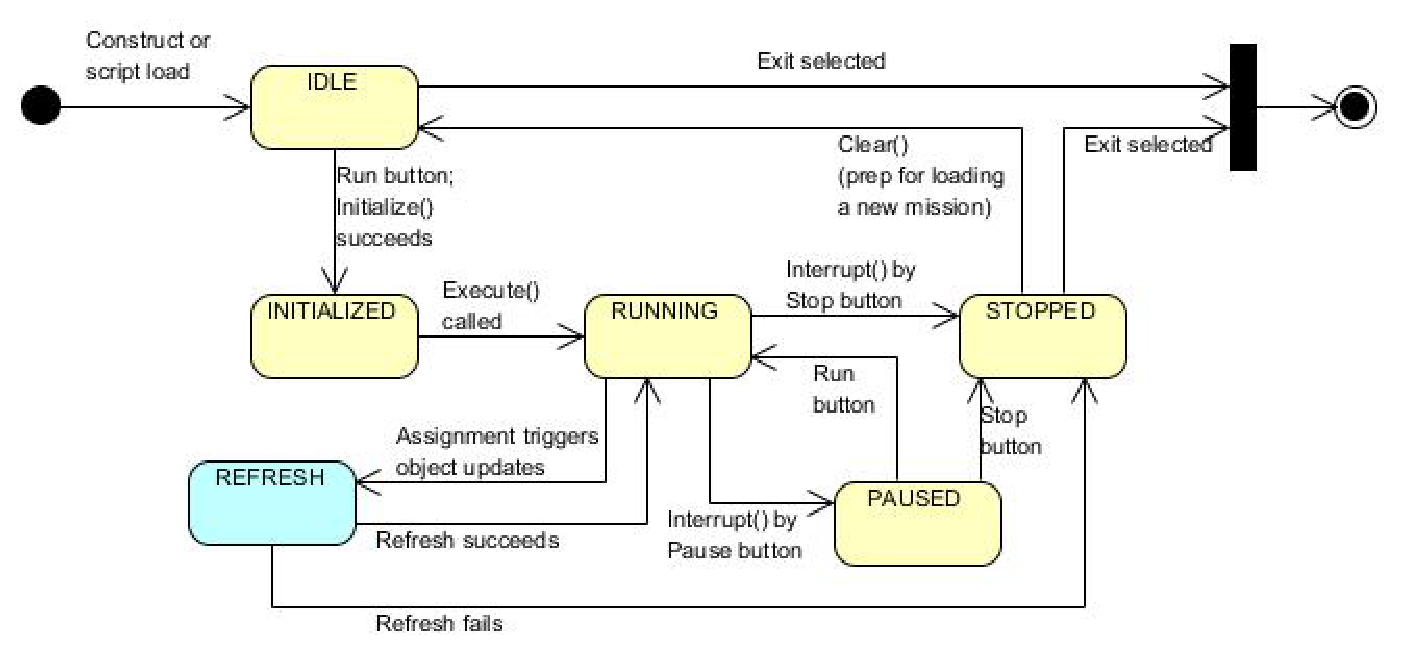
\includegraphics[scale=0.6]{Images/SandboxStateTransitions-updated.eps}
\caption{\label{figure:SandboxStates}Initialization of a Control Sequence in the Sandbox}
\end{center}
\end{figure}

GMAT's Sandbox implements a finite state machine that manages mission runs.  Figure~\ref{figure:SandboxStates} shows the state transitions performed in the Sandbox during a run.  The REFRESH state, colored cyan in the figure, is of particular interest to the current discussion.  When a GMAT Sandbox executes an Assignment command in the Mission Control Sequence, the Sandbox transitions into the REFRESH state if a configured object was updated so that hidden clones of that object can receive the new object data and be reinitialized when necessary.  Upon this state transition, GMAT control flow for the Sandbox follows the process illustrated in the top portion of Figure~\ref{figure:SandboxReinitialization}:

\begin{figure}[htb]
\begin{center}
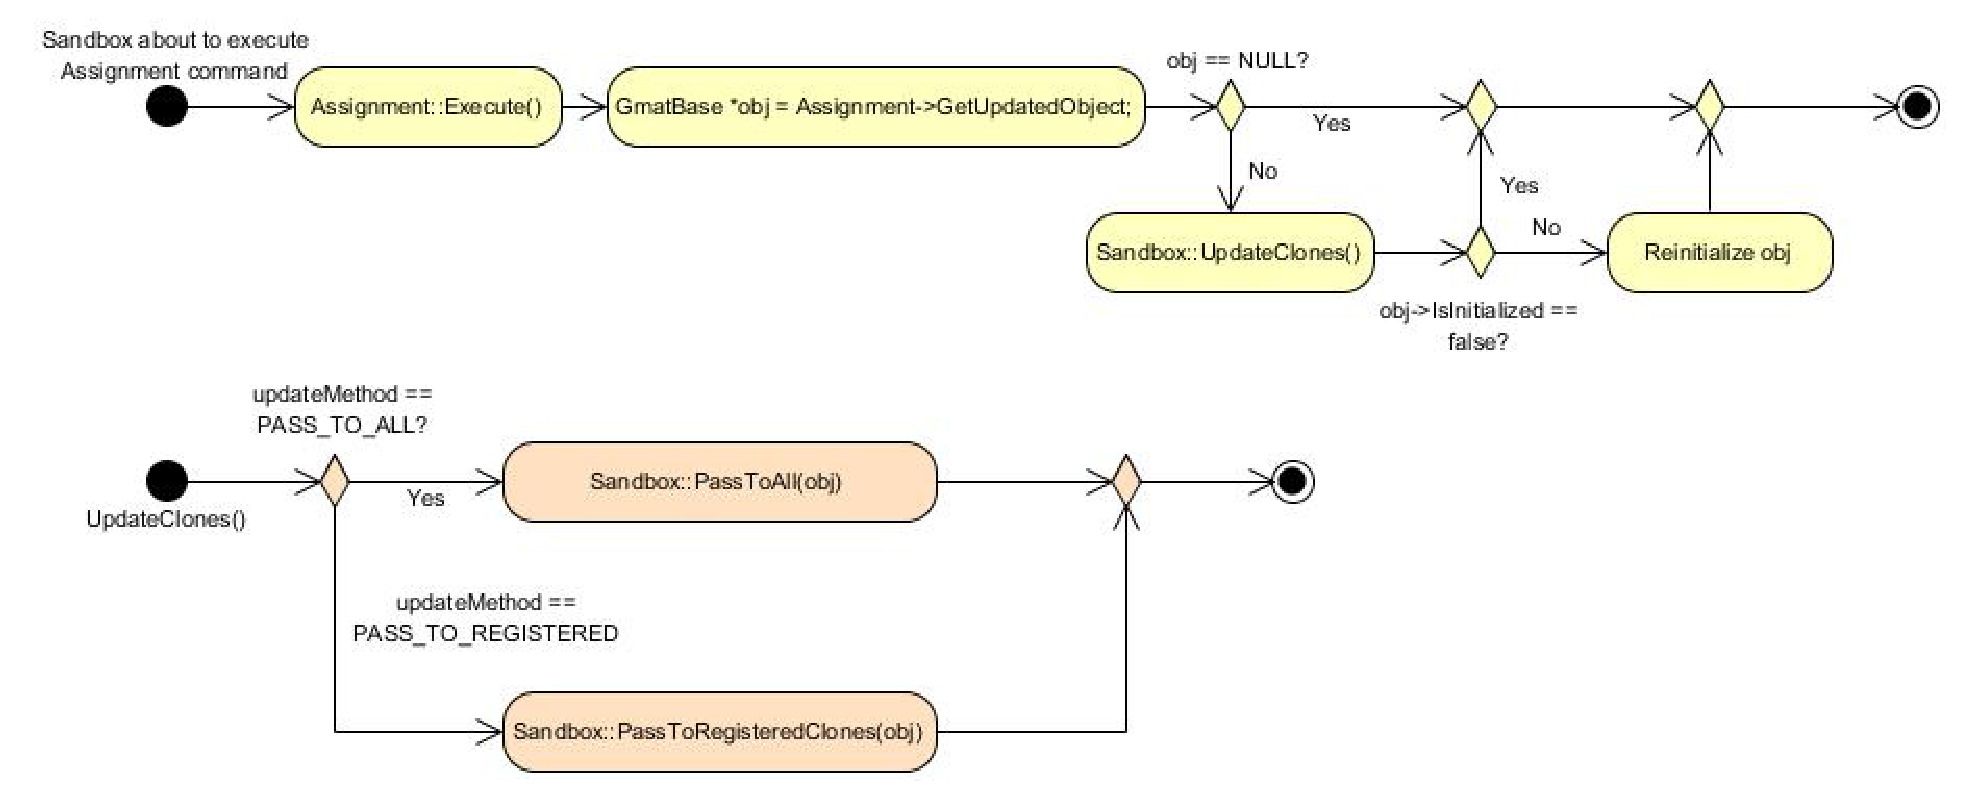
\includegraphics[scale=0.5]{Images/SandboxCloneUpdates.eps}
\caption{\label{figure:SandboxReinitialization}Clone Updating and Initialization During a Run}
\end{center}
\end{figure}

\begin{itemize}
\item The Assignment command is executed
\item The Assignment command passes the updated object pointer to the Sandbox
\item If the returned object is not NULL, the Sandbox changes state to the REFRESH state (see Figure~\ref{figure:SandboxStates}) and control passes to the UpdateClones() method
\item The UpdateClones() method calls an update method based on the updateMethod selection, as is shown in the lower diagram in Figure~\ref{figure:SandboxReinitialization} 
\item Reinitialize the updated object
\end{itemize}

Figure~\ref{figure:PassToAllDetails} shows the process implemented in the PassToAll() method for clone updates.  This method passes clone data to every user object in the Sandbox, giving each the opportunity to receive data for owned clones.  The procedure followed by this method is:

\begin{figure}[htb]
\begin{center}
\includegraphics[scale=0.5]{Images/SandboxClonePassToAll.eps}
\caption{\label{figure:PassToAllDetails}Clone Updating Using the PassToAll() method}
\end{center}
\end{figure}

\begin{itemize}
\item The Sandbox passes the updated object to each object in the local object store so that local clones can copy the new data into their local clones
\item If a clone was updated, it is immediately reinitialized if reinitialization is necessary
\item The Sandbox passes the updated object to each object in the global object store so that local clones can copy the new data into their local clones
\item If a clone was updated, it is immediately reinitialized if reinitialization is necessary
\item The Sandbox passes the updated object to each command in the Mission Control Sequence so that local clones can copy the new data into their local clones
\item If a clone was updated, it is immediately reinitialized if reinitialization is necessary
\end{itemize}

\noindent The basic process, repeated for each of the three target collections of objects (The local object store, the global object store, and the Mission Control Sequence) is to

\begin{enumerate}
\item Start at the beginning of the collection
\item Pass the updated object into the UpdateClonedObject() method, which applies the assignment operator to pass the new data to any clone of the object
\item Check to see if the objects need reinitialization, and reinitialize as needed
\item Retrieve the next object in the collection
\item Repeat the process until all members of the collect have had the opportunity to receive the new data for local clones
\end{enumerate}

\noindent The portion of this process associated with the commands in the Mission Control Sequence is slightly more complex than is shown in the figure when the command is a BranchCommand.  The BranchCommand class walks its branch control sequence, performing the clone management tasks for each command in the branch sequence in turn as part of the UpdateClonedObject() method.  Once all of the object collections have received the updated object for their clones, that object is reinitialized when necessary, completing the process.  Objects that do not have local clones use the default implementation of the UpdateClonedObject() method, which just returns false to indicate that no local clones were updated.

The second option, PassToRegisteredClones, is more efficient.  It registers local clone objects as they are loaded into the Sandbox, and uses that registration to pass the clone data into the registered clones.  The details of that approach will be specified when the approach is implemented. 

\end{document}